This problem is meant to introduce you to \emph{hat} functions, which will form the basis (double meaning intented) of the finite element method.

Let $f\in C[0,1]$ be such that $f(x) = \sin(\pi x)$. Suppose that $N$ is a positive integer and define $\displaystyle{h = {1\over N+1}}$ and $x_j = jh$ for $j = 0,1\ldots, N+1$. Consider the $N$ hat functions $\phi_k\in C[0,1]$, defined as
\[
\phi_k(x) = \left\{
\begin{array}{ll}
\displaystyle{{x-x_{k-1}\over h}} & \mbox{if }x\in [x_{k-1}, x_k);\\
\displaystyle{{x_{k+1}-x\over h}} & \mbox{if }x\in [x_k, x_{k+1});\\
0 & \mbox{otherwise};
\end{array}\right.
\]
for $k=1,\ldots, N$. We call these piecewise linear functions {\em hat functions} 
because of their shape.  
As an example, when $N=9$ and $k=3$, this function takes the following form.
\begin{center}
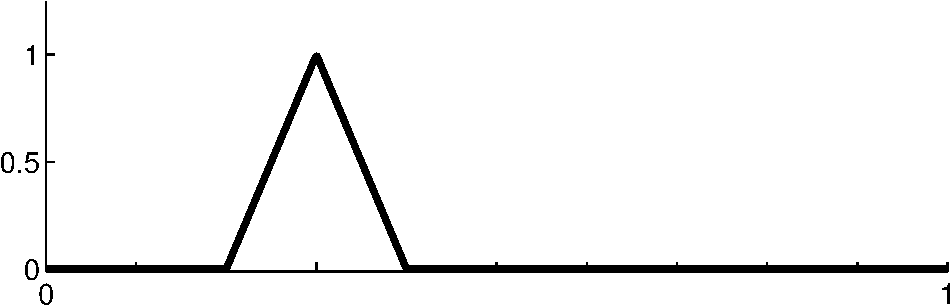
\includegraphics[scale=0.6]{plothat}
\begin{picture}(0,0)
\put(-215,0){$x_2$}
\put(-190,0){$x_3$}
\put(-165,0){$x_4$}
\put(-175,50){$\phi_3(x)$}
\end{picture}
\end{center}


Let the inner product $\ip{\cdot,\cdot}:\mbox{ }C[0,1]\times C[0,1]\rightarrow\R$ be defined by
\[
\ip{u,v} = \int_0^1 u(x)v(x)\, dx
\]
and let the norm $\norm{\cdot}:\mbox{ }C[0,1]\rightarrow\R$ be defined by
\[
\norm{u} = \sqrt{\ip{u,u}}.
\]
\\
\begin{enumerate}
\item For $j=1,\ldots,N$, what is $\phi_j(x_k)$ for $k=0,1,\ldots,N+1$? Simplify your answer as much as possible.
\\
\item Show that $\{\phi_1, \ldots, \phi_N\}$ is linearly independent by showing that if $c_k\in\mathbb{R}$ and $\displaystyle{\sum_{k=1}^N}c_k\phi_k(x)=0$ for all $x\in[0,1]$ then $c_k=0$ for $k=1,\ldots,N$.
\\
\item By hand, compute $(f,\phi_j)$ for $j=1,\ldots, N$.
\\
\item By hand, compute $(\phi_j, \phi_k)$ for $j,k=1,\ldots, N$. Your final answers should be simplified as much as possible and in your formulas $h$ should be left as $h$ and not be replaced with $1/(N+1)$. You must clearly state which values of $j$ and $k$ each formula you obtain is valid for. An acceptable way to present the final answer would be:\newline
For $j,k=1,\ldots,N$,
\[
\ip{\phi_j,\phi_k}=\left\{\begin{array}{ll}? & \mbox{if }k=j, \\[.75em] ? & \mbox{if }\left|j-k\right|=1, \\[.75em] ? & \mbox{otherwise},\end{array}\right.
\]
with the question marks replaced with the correct values. Hint: Letting $s=x-x_{j-1}$ yields that
\[
\int_{x_{j-1}}^{x_j}\left({x-x_{j-1}\over h}\right)^2\,dx={1 \over h^2}\int_{x_{j-1}-x_{j-1}}^{x_j-x_{j-1}}\left(s+x_{j-1}-x_{j-1}\right)^2\,ds={1 \over h^2}\int_0^hs^2\,ds.
\]
\\
\item Set up a linear system (in MATLAB) and solve it to compute the best approximation $f_N$ to $f$ from ${\rm span}\{\phi_1, \ldots, \phi_N\}$  with respect to the norm $\norm{\cdot}$ for $N=3$ and $N=9$. For each of these $N$, produce a separate plot that superimposes $f_N(x)$ on top of a plot of $f(x)$. The \verb|hat.m| code 
%(from Homework~2, either your code or the code from the solutions) 
should help you to produce these plots.

\end{enumerate}

%%%%%%%%%%%%%%%%%%%%%%%%%%%%%%%%%%%%%%%%%%%%%%%%%%%%%%%%%%%%%%%%%%%%%%%%%%%%%%%%

\ifthenelse{\boolean{showsols}}{\input hats_sol}{}

